\documentclass[DM,authoryear,toc]{lsstdoc}
% lsstdoc documentation: https://lsst-texmf.lsst.io/lsstdoc.html
\input{meta}

% Package imports go here.

% Local commands go here.

%If you want glossaries
%\input{aglossary.tex}
%\makeglossaries

\title{Node Utilization for HSC-RC2 Reprocessing Jobs}

% Optional subtitle
% \setDocSubtitle{A subtitle}

\author{%
Samantha Thrush
}

\setDocRef{DMTN-161}
\setDocUpstreamLocation{\url{https://github.com/lsst-dm/dmtn-161}}

\date{8 May 2018}

% Optional: name of the document's curator
% \setDocCurator{The Curator of this Document}

\setDocAbstract{%
  Summary of node utilization for RC2 jobs between \texttt{w\_2018\_04} and \texttt{w\_2018\_18} releases as presented on the Node Utilization for HSC-RC2 Reprocessing Jobs Confluence page (\url{https://confluence.lsstcorp.org/pages/viewpage.action?spaceKey=~sthrush&title=Node+Utilization+for++HSC-RC2+Reprocessing+Jobs}).
}

% Change history defined here.
% Order: oldest first.
% Fields: VERSION, DATE, DESCRIPTION, OWNER NAME.
% See LPM-51 for version number policy.
\setDocChangeRecord{%
  \addtohist{1}{YYYY-MM-DD}{Unreleased.}{Hsin-Fang Chiang}
}


\begin{document}

% Create the title page.
\maketitle
% Frequently for a technote we do not want a title page  uncomment this to remove the title page and changelog.
% use \mkshorttitle to remove the extra pages

% ADD CONTENT HERE
% You can also use the \input command to include several content files.
This document collects notes about the HyprSuprime Cam Release Candidate 2 (HSC RC2) reprocessing in cycle S18.

Description of the HSC RC2 processing can be found in \citeds{DMTN-088}.
Summary of all individual HSC RC2 reprocessing runs from \texttt{w\_2018\_04} to \texttt{w\_2020\_34} can be found in the Reprocessing of the HSC RC2 Dataset Confluence notes: \url{https://confluence.lsstcorp.org/display/DM/Reprocessing+of+the+HSC+RC2+dataset}.
The definition of HSC RC2 dataset is given in \jira{DM-11345}.

This document summarizes version 04, 06, 08, 10, 12, 14, 15, 17, 18 reprocessing runs. SLURM ids of runs are defined in \jira{DM-14056}.

All of the plots were created with \texttt{usage.py} (see \url{https://github.com/lsst-dm/ldf\_ops\_tools}) and were assigned a resolution of 8000 so as to make sure to catch any short jobs.
The node-hours and the elapsed run times do not depend on the resolution, as they re extracted directly from the SLURM accounting data.


\clearpage
\section{Summary of node utilization across releases}
\begin{table}[h]
  \centering
  \begin{tabular} {|c|c|}
    \hline
    Release & Node-hours \\
    \hline
    w\_2018\_04 & 251.03 \\
    w\_2018\_06 & 347.61 \\
    w\_2018\_08 & 539.88 \\
    w\_2018\_10 & 890.82 \\
    w\_2018\_12 & 683.69 \\
    w\_2018\_14 & 540.95 \\
    w\_2018\_15 & 530.26 \\
    w\_2018\_17 & 513.39 \\
    w\_2018\_18 & 473.86 \\
    \hline
  \end{tabular}
  \caption{Summary of node-hours for all weekly release version of interest.}
  \label{SummaryTable}
\end{table}

\begin{figure}[h]
  \centering
  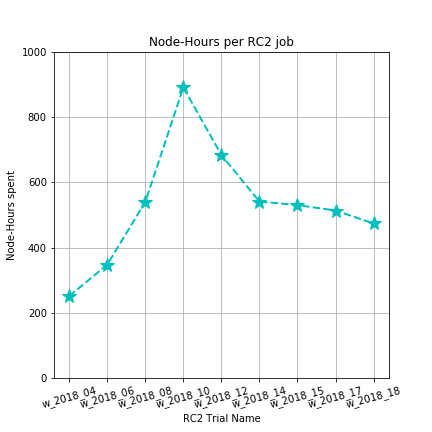
\includegraphics[width=0.70\textwidth]{figures/RC2_nodehours.png}
  \caption{Node-hours usage across different releases.}
  \label{SummaryFig}
\end{figure}

\clearpage
\section{Node utilization per processing step for release w\_2018\_04}
\begin{table}[h]
  \centering
  \begin{tabular} {|c|c|}
    \hline
    Processing step & Node-hours \\
    \hline
    SingleFrameDriver &  71.59 \\ 
    MakeSkyMap        &   0.02 \\
    Mosaic            &   6.37 \\
    SkyCorrection     &   0.00 \\
    CoaddDriver       &  31.44 \\
    MultibandDriver   & 141.61 \\
    \hline
  \end{tabular}
  \caption{Summary of node-hours for all weekly release version w\_2018\_04}
  \label{tbl:PerTask04}
\end{table}

\begin{figure}[h]
  \centering
  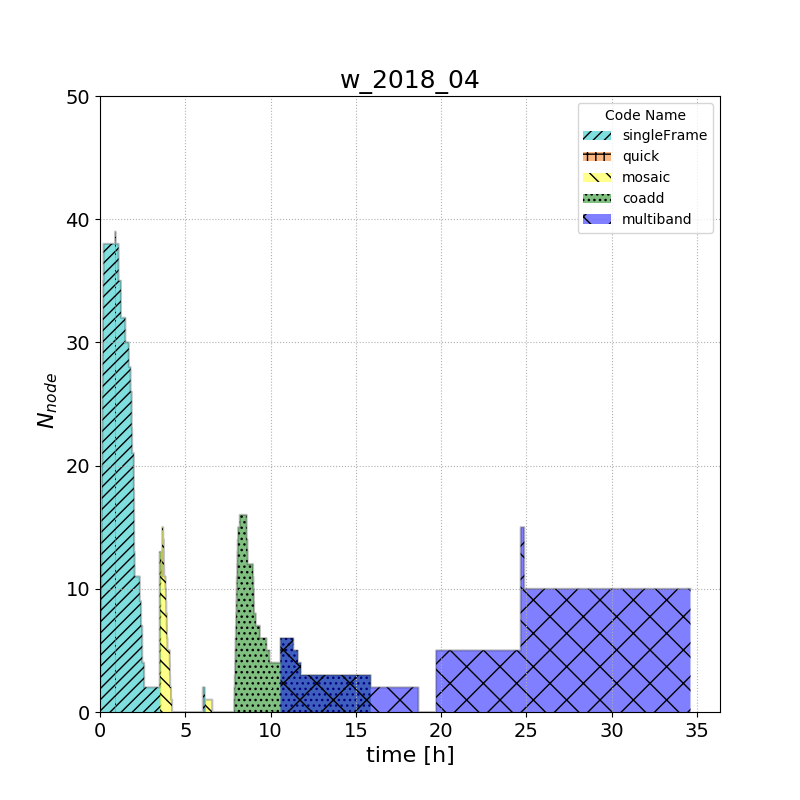
\includegraphics[width=0.70\textwidth]{figures/usage-w_2018_04-ultimate.png}
  \caption{Node-hours usage per processing step for w\_2018\_04}
  \label{fig:PerTask04}
\end{figure}


\clearpage
\section{Node utilization per processing step for release w\_2018\_06}
\begin{table}[h]
  \centering
  \begin{tabular} {|c|c|}
    \hline
    Processing step & Node-hours \\
    \hline
    SingleFrameDriver &  92.52 \\ 
    MakeSkyMap        &   0.01 \\
    Mosaic            &  18.61 \\
    SkyCorrection     &  11.73 \\
    CoaddDriver       &  31.44 \\
    MultibandDriver   & 192.29 \\
    \hline
  \end{tabular}
  \caption{Summary of node-hours for all weekly release version w\_2018\_06}
  \label{tbl:PerTask06}
\end{table}

\begin{figure}[h]
  \centering
  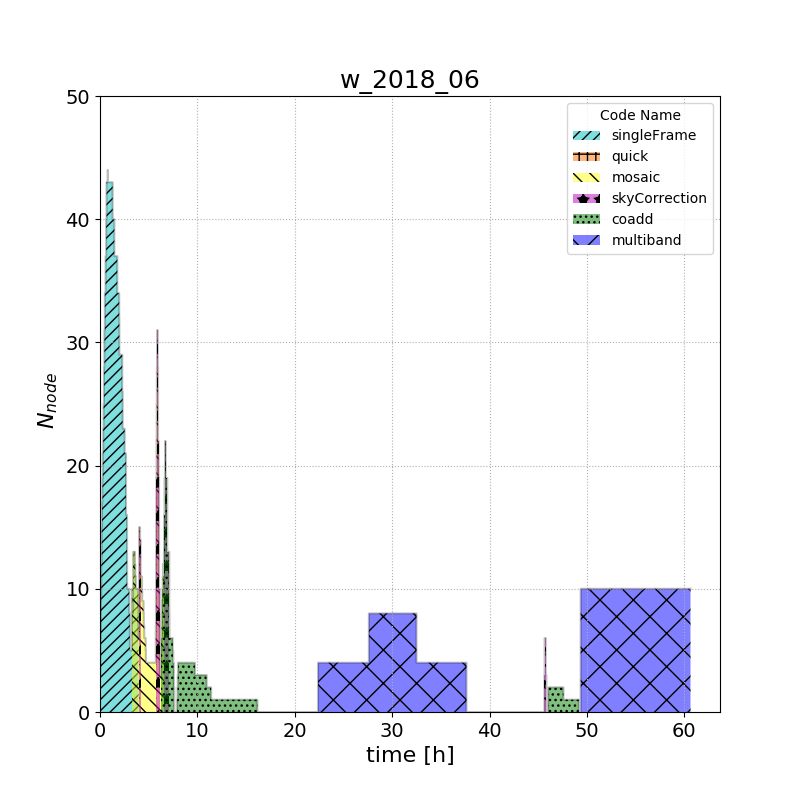
\includegraphics[width=0.70\textwidth]{figures/usage-w_2018_06-ultimate.png}
  \caption{Node-hours usage per processing step for w\_2018\_06}
  \label{fig:PerTask06}
\end{figure}


\clearpage
\section{Node utilization per processing step for release w\_2018\_08}
\begin{table}[h]
  \centering
  \begin{tabular} {|c|c|}
    \hline
    Processing step & Node-hours \\
    \hline
    SingleFrameDriver &  83.86 \\ 
    MakeSkyMap        &   0.02 \\
    Mosaic            &  32.66 \\
    SkyCorrection     &  15.36 \\
    CoaddDriver       &  42.70 \\
    MultibandDriver   & 365.28 \\
    \hline
  \end{tabular}
  \caption{Summary of node-hours for all weekly release version w\_2018\_08}
  \label{tbl:PerTask08}
\end{table}

\begin{figure}[h]
  \centering
  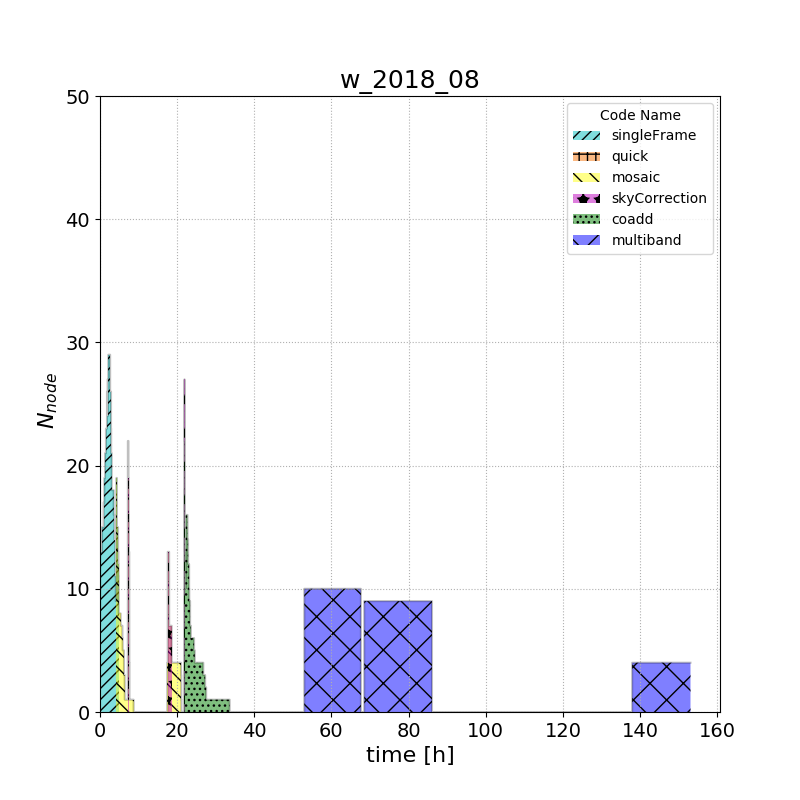
\includegraphics[width=0.70\textwidth]{figures/usage-w_2018_08-ultimate.png}
  \caption{Node-hours usage per processing step for w\_2018\_08}
  \label{fig:PerTask08}
\end{figure}


\clearpage
\section{Node utilization per processing step for release w\_2018\_10}
\begin{table}[h]
  \centering
  \begin{tabular} {|c|c|}
    \hline
    Processing step & Node-hours \\
    \hline
    SingleFrameDriver &  81.81 \\ 
    MakeSkyMap        &   0.02 \\
    Mosaic            &   5.39 \\
    SkyCorrection     &   7.66 \\
    CoaddDriver       &  42.00 \\
    MultibandDriver   & 753.94 \\
    \hline
  \end{tabular}
  \caption{Summary of node-hours for all weekly release version w\_2018\_10}
  \label{tbl:PerTask10}
\end{table}

\begin{figure}[h]
  \centering
  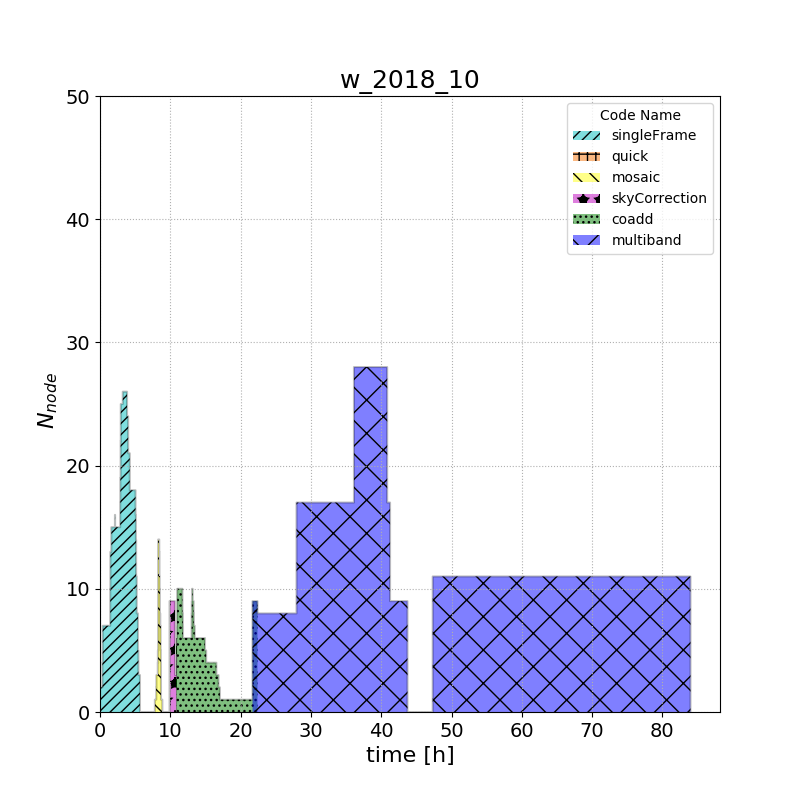
\includegraphics[width=0.70\textwidth]{figures/usage-w_2018_10-ultimate.png}
  \caption{Node-hours usage per processing step for w\_2018\_10}
  \label{fig:PerTask10}
\end{figure}


\clearpage
\section{Node utilization per processing step for release w\_2018\_12}
\begin{table}[h]
  \centering
  \begin{tabular} {|c|c|}
    \hline
    Processing step & Node-hours \\
    \hline
    SingleFrameDriver &  80.22 \\ 
    MakeSkyMap        &   0.02 \\
    Mosaic            &   5.08 \\
    SkyCorrection     &   7.23 \\
    CoaddDriver       &  33.31 \\
    MultibandDriver   & 557.83 \\
    \hline
  \end{tabular}
  \caption{Summary of node-hours for all weekly release version w\_2018\_12}
  \label{tbl:PerTask12}
\end{table}

\begin{figure}[h]
  \centering
  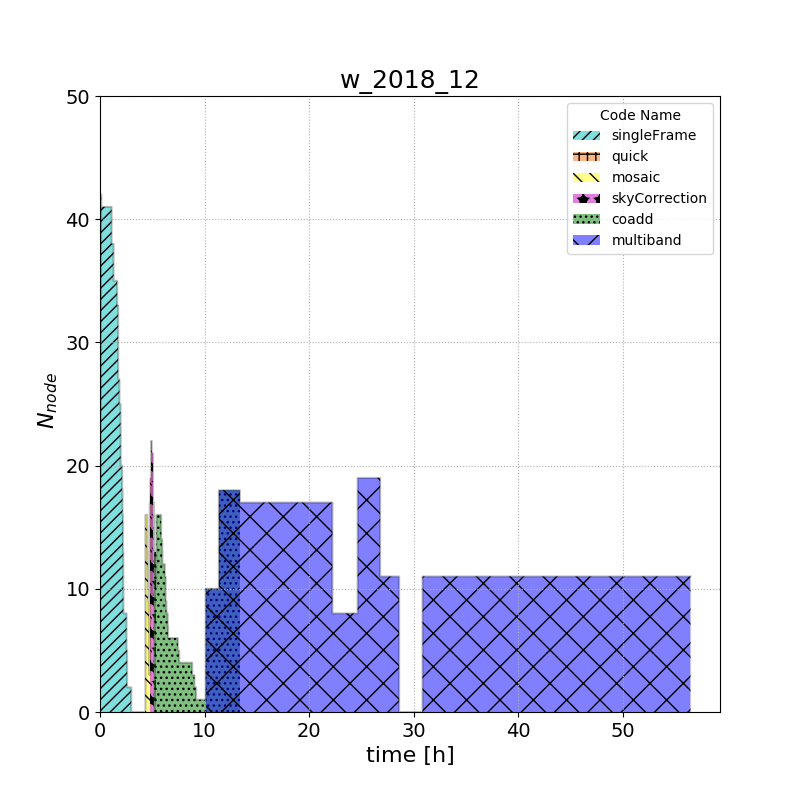
\includegraphics[width=0.70\textwidth]{figures/usage-w_2018_12-ultimate.png}
  \caption{Node-hours usage per processing step for w\_2018\_12}
  \label{fig:PerTask12}
\end{figure}


\clearpage
\section{Node utilization per processing step for release w\_2018\_14}
\begin{table}[h]
  \centering
  \begin{tabular} {|c|c|}
    \hline
    Processing step & Node-hours \\
    \hline
    SingleFrameDriver &  79.38 \\ 
    MakeSkyMap        &   0.02 \\
    Mosaic            &  10.97 \\
    SkyCorrection     &  20.38 \\
    CoaddDriver       &  37.16 \\
    MultibandDriver   & 393.04 \\
    \hline
  \end{tabular}
  \caption{Summary of node-hours for all weekly release version w\_2018\_14}
  \label{tbl:PerTask14}
\end{table}

\begin{figure}[h]
  \centering
  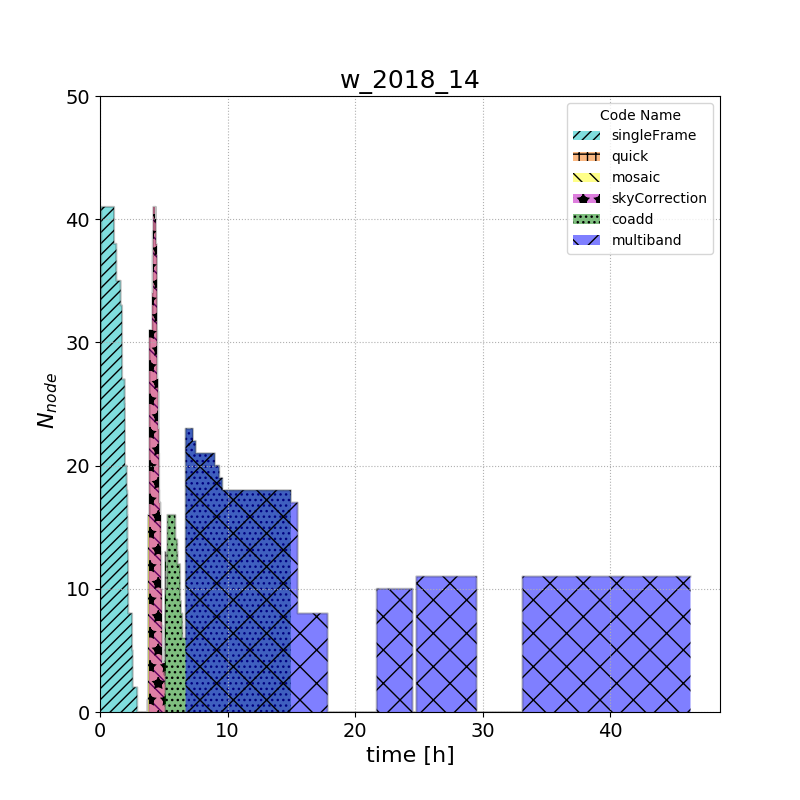
\includegraphics[width=0.70\textwidth]{figures/usage-w_2018_14-ultimate.png}
  \caption{Node-hours usage per processing step for w\_2018\_14}
  \label{fig:PerTask14}
\end{figure}


\clearpage
\section{Node utilization per processing step for release w\_2018\_15}
\begin{table}[h]
  \centering
  \begin{tabular} {|c|c|}
    \hline
    Processing step & Node-hours \\
    \hline
    SingleFrameDriver &  73.64 \\ 
    MakeSkyMap        &   0.03 \\
    Mosaic            &  10.44 \\
    SkyCorrection     &  16.50 \\
    CoaddDriver       &  36.67 \\
    MultibandDriver   & 392.99 \\
    \hline
  \end{tabular}
  \caption{Summary of node-hours for all weekly release version w\_2018\_15}
  \label{tbl:PerTask15}
\end{table}

\begin{figure}[h]
  \centering
  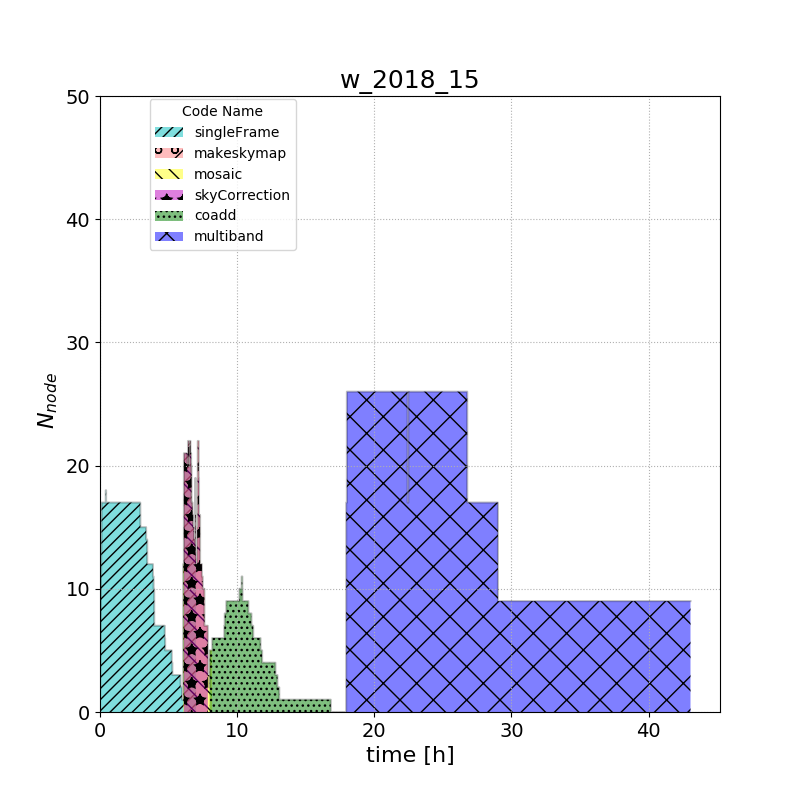
\includegraphics[width=0.70\textwidth]{figures/usage-w_2018_15.png}
  \caption{Node-hours usage per processing step for w\_2018\_15}
  \label{fig:PerTask15}
\end{figure}


\clearpage
\section{Node utilization per processing step for release w\_2018\_17}
\begin{table}[h]
  \centering
  \begin{tabular} {|c|c|}
    \hline
    Processing step & Node-hours \\
    \hline
    SingleFrameDriver &  78.86 \\ 
    MakeSkyMap        &   0.02 \\
    Mosaic            &   5.24 \\
    SkyCorrection     &   7.01 \\
    CoaddDriver       &  29.51 \\
    MultibandDriver   & 392.75 \\
    \hline
  \end{tabular}
  \caption{Summary of node-hours for all weekly release version w\_2018\_17}
  \label{tbl:PerTask17}
\end{table}

\begin{figure}[h]
  \centering
  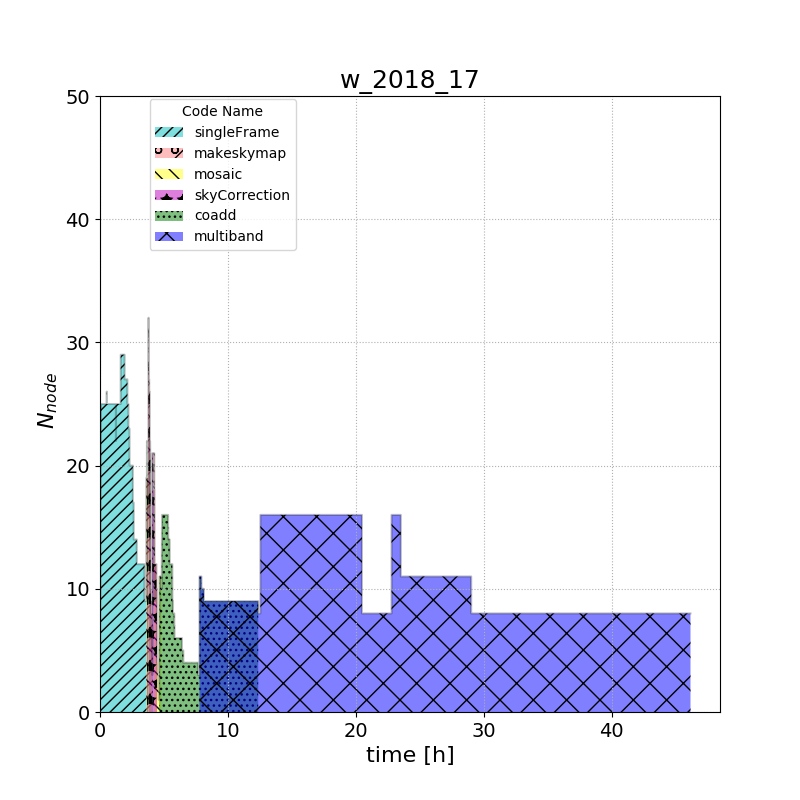
\includegraphics[width=0.70\textwidth]{figures/usage-w_2018_17.png}
  \caption{Node-hours usage per processing step for w\_2018\_17}
  \label{fig:PerTask17}
\end{figure}


\clearpage
\section{Node utilization per processing step for release w\_2018\_18}
\begin{table}[h]
  \centering
  \begin{tabular} {|c|c|}
    \hline
    Processing step & Node-hours \\
    \hline
    SingleFrameDriver &  92.09 \\ 
    MakeSkyMap        &   0.02 \\
    Mosaic            &   5.67 \\
    SkyCorrection     &   4.41 \\
    CoaddDriver       &  27.70 \\
    MultibandDriver   & 343.98 \\
    \hline
  \end{tabular}
  \caption{Summary of node-hours for all weekly release version w\_2018\_18}
  \label{tbl:PerTask18}
\end{table}

\begin{figure}[h]
  \centering
  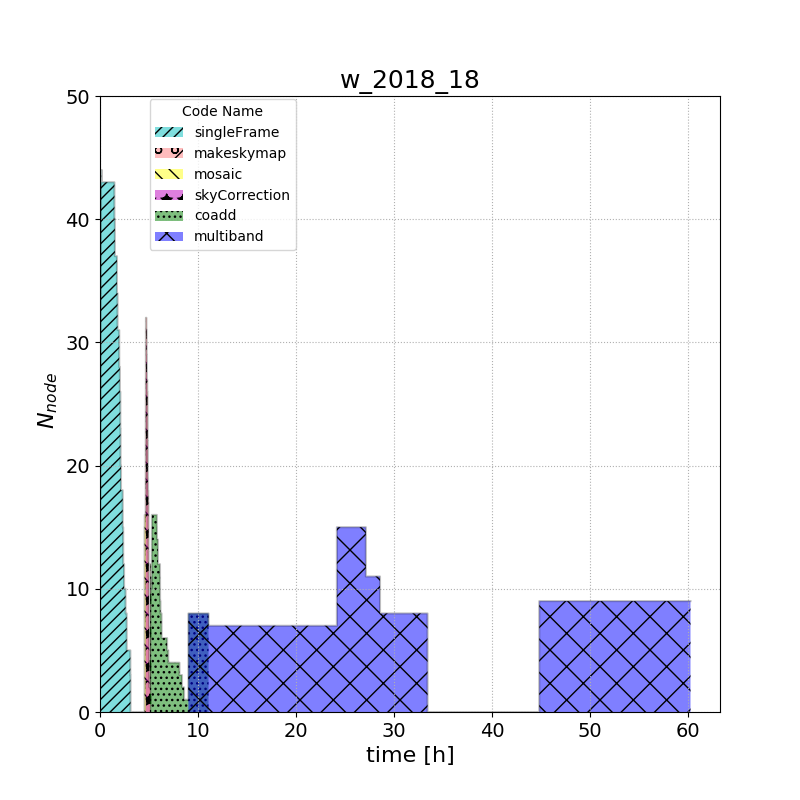
\includegraphics[width=0.70\textwidth]{figures/usage-w_2018_18.png}
  \caption{Node-hours usage per processing step for w\_2018\_18}
  \label{fig:PerTask18}
\end{figure}


\appendix
% Include all the relevant bib files.
% https://lsst-texmf.lsst.io/lsstdoc.html#bibliographies
\section{References} \label{sec:bib}
\renewcommand{\refname}{} % Suppress default Bibliography section
\bibliography{local,lsst,lsst-dm,refs_ads,refs,books}

% Make sure lsst-texmf/bin/generateAcronyms.py is in your path
\section{Acronyms} \label{sec:acronyms}
\addtocounter{table}{-1}
\begin{longtable}{p{0.145\textwidth}p{0.8\textwidth}}\hline
\textbf{Acronym} & \textbf{Description}  \\\hline

 &  \\\hline
DM & Data Management \\\hline
DMTN & DM Technical Note \\\hline
HSC & Hyper Suprime-Cam \\\hline
\end{longtable}

% If you want glossary uncomment below -- comment out the two lines above
%\printglossaries





\end{document}
